\documentclass[12pt,a4paper]{article}

% -------- PACKAGES --------
\usepackage[utf8]{inputenc}
\usepackage[T1]{fontenc}
\usepackage{graphicx}
\usepackage{geometry}
\usepackage{hyperref}
\usepackage{listings}
\usepackage{xcolor}
\usepackage{titlesec}
\usepackage{caption}

\geometry{margin=1in}

% -------- COLORS & LINKS --------
\definecolor{codegray}{rgb}{0.95,0.95,0.95}
\hypersetup{
    colorlinks=true,
    linkcolor=blue,
    urlcolor=cyan,
    pdftitle={EV Charging Simulation Report}
}

% -------- CODE STYLE --------
\lstset{
    backgroundcolor=\color{codegray},
    basicstyle=\ttfamily\footnotesize,
    frame=single,
    breaklines=true,
    postbreak=\mbox{\textcolor{red}{$\hookrightarrow$}\space}
}

% -------- TITLE --------
\title{
    \vspace{3cm}
    \textbf{EV Charging Simulation}\\
    \large Development, Deployment and Results Report\\
    \vspace{1cm}
}
\author{
    Your Name\\
    \texttt{your.email@example.com}\\
    Institution / Course Name
}
\date{\today}

\begin{document}

\maketitle
\newpage
\tableofcontents
\newpage

% ======================================================
\section{Executive Summary}
This project implements a distributed Electric Vehicle (EV) charging simulation platform using mainly 
Python, Apache Kafka, and Docker.
It models the interactions between a central management service, multiple charging points (CP) with engines, monitors supervising the state of engines,
and driver applications.
All services are containerized and orchestrated via Docker Compose, 
enabling reproducible deployment and communication through Kafka topics, TCP sockets, and HTTP endpoints.

% ======================================================
\section{System Architecture}

\subsection{Overview}
Architecture used in this system is microservice-based architecture. 
It can be observed in the fact that all the components run independently and are event-driven.
The system contains numerous crucial components which communicate with each other thanks to Kafka and TCP sockets.
The main objective of this system is to simulate real-world EV chargin system.
In the reality it is almost impossible to mantain manual controll over every component of such system
with all plausible faults or user's errors.
Our architecture tries to automate the process of communication between components and prepare the system
for the unpredictability of an outside world.

\subsection{Architecture Diagram}
\begin{figure}[h!]
    \centering
    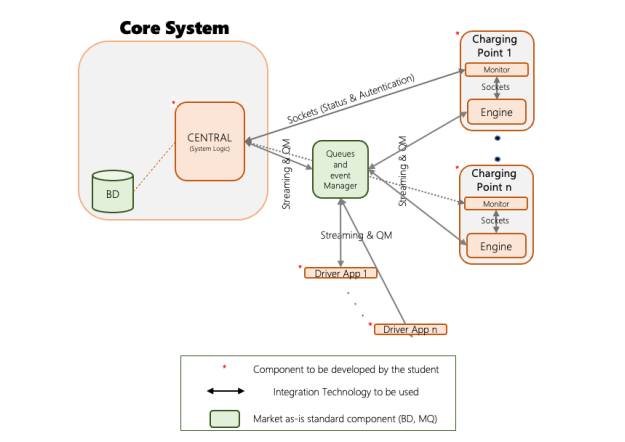
\includegraphics[width=0.9\textwidth]{architecture.png}
    \caption{Architecture of the EV Charging Simulation system.}
\end{figure}

\subsection{Components Description}
\begin{table}[h!]
\centering
\begin{tabular}{|l|l|l|l|}
\hline
\textbf{Component} & \textbf{Role} & \textbf{Technology} & \textbf{Port} \\ \hline
Central & Manages registration, commands, and telemetry & FastAPI, aiokafka & 8000 \\ \hline
CP Engine & Simulates charging session & Python, Kafka, Sockets & 8001 \\ \hline
CP Monitor & Monitors Engine and reports to Central & Python, HTTP, Sockets & -- \\ \hline
Driver & Simulates driver requests & FastAPI, Python, Kafka & -- \\ \hline
Kafka & Message broker & Apache Kafka & 9092 \\ \hline
\end{tabular}
\caption{System components and their technologies.}
\end{table}
Responsibilities of each component:
\begin{itemize}
    \item Central:
        \begin{itemize}
            \item Acts as the central controller and coordinator
            \item Provides a FastAPI dashboard for readability
            \item Receives registration requests from new CP Monitors
            \item Receives heartbeats from the CP Monitors
            \item Receives fault/health notifications
            \item Stores state about all charging points 
        \end{itemize}
    \item CP Monitor:
        \begin{itemize}
            \item Oversees a single CP Engine's health and connectivity
            \item Sends heartbeats to the Central
            \item Performs TCP healthcheck against the CP Engine
            \item Notifies Central of faults
            \item Registes with the Central at startup
        \end{itemize}
    \item CP Engine:
        \begin{itemize}
            \item Simulates the physical charging point
            \item Publishes telemetry messages to Kafka topics
            \item Listens for start/stop requests
            \item Provides a TCP health endpoint for the Monitor
        \end{itemize}
    \item Kafka:
        \begin{itemize}
            \item Simulates the physical charging point
            \item Publishes telemetry messages to Kafka topics
            \item Listens for start/stop requests
            \item Provides a TCP health endpoint for the Monitor
        \end{itemize}
    \item Docker:
        \begin{itemize}
            \item Simulates the physical charging point
            \item Publishes telemetry messages to Kafka topics
            \item Listens for start/stop requests
            \item Provides a TCP health endpoint for the Monitor
        \end{itemize}
    \item Data base:
        \begin{itemize}
            \item Simulates the physical charging point
            \item Publishes telemetry messages to Kafka topics
            \item Listens for start/stop requests
            \item Provides a TCP health endpoint for the Monitor
        \end{itemize}
\end{itemize}


% ======================================================
\section{Development Process}

\subsection{Environment Setup}
List tools and libraries used (Python 3.11, Kafka 3.7, Docker, etc.).

\subsection{Repository Structure}
\begin{lstlisting}
ev-charging-simulation/
|-- docker/
|   |-- Dockerfile.central
|   |-- Dockerfile.cp_e
|   |-- Dockerfile.cp_m
|   |-- Dockerfile.driver
|-- docker-compose.yml
|-- Makefile
`-- evcharging/
    |-- apps/
    |   |-- ev_central/
    |   |-- ev_cp_e/
    |   |-- ev_cp_m/
    |   `-- ev_driver/
    `-- common/
\end{lstlisting}

\subsection{Key Features}
\begin{itemize}
    \item Asynchronous Kafka-based communication.
    \item State management using Python enumerations.
    \item Health endpoints via FastAPI.
    \item Docker Compose-based deployment and inter-service networking.
\end{itemize}

% ======================================================
\section{Deployment Details}

\subsection{Docker Setup}
Explain the purpose of each Dockerfile and the role of docker-compose.

\begin{lstlisting}[caption={Excerpt from docker-compose.yml}]
services:
  ev-central:
    build:
      context: .
      dockerfile: docker/Dockerfile.central
    ports:
      - "8000:8000"
    depends_on:
      kafka:
        condition: service_healthy
\end{lstlisting}

\subsection{Health Checks}
Describe how health checks are implemented (via curl, nc, etc.).

\subsection{Kafka Topics}
List topics such as:
\begin{itemize}
    \item central.commands
    \item cp.telemetry
    \item cp.status
    \item driver.requests
\end{itemize}

% ======================================================
\section{Testing and Results}

\subsection{Testing Procedure}
Describe how containers were launched, logs monitored, and communication verified.

\subsection{Example Logs}
\begin{lstlisting}
INFO: CP cp-1 registered with Central successfully
INFO: Received telemetry update for cp-1
INFO: Driver command processed successfully
\end{lstlisting}

\subsection{Results}
Summarize key outcomes (successful registration, telemetry flow, driver interaction).

% ======================================================
\section{Troubleshooting and Corrections}

Document encountered issues and solutions:
\begin{itemize}
    \item Fixed missing wait-for-kafka script.
    \item Added curl to support health checks.
    \item Adjusted Kafka listener configuration.
\end{itemize}

% ======================================================
\section{Conclusion}

Summarize the project outcomes, limitations, and future improvements (e.g. database persistence, dashboard UI).

% ======================================================
\appendix
\section{Appendices}

\subsection{Run Instructions}
\begin{lstlisting}
docker compose build
docker compose up
\end{lstlisting}

\subsection{Sample API Endpoints}
\begin{itemize}
    \item \texttt{GET /health}
    \item \texttt{POST /cp/register}
\end{itemize}

\end{document}
